\documentclass[00-main.tex]{subfiles}

\begin{document}

\chapter{Preparation}

In this chapter I describe my research into the WebAssembly architecture and the Relooper algorithm, and highlight the main features of Rust, the programming language I learnt for this project, and my rationale for using it.

Furthermore, I discuss the requirements of the project, and describe the software engineering approach I employed, before outlining my starting point and previous experience.

\section{WebAssembly}

Initially, I extensively researched the WebAssembly specification to gain a deep understanding of the target binary code~\ccite{wasm-spec}.
The following sections provide an overview of the instruction set architecture.

\subsection{Primitive Values}

\Ccref{tab:wasm value types} below outlines the primitive values supported by WebAssembly.
Booleans and memory addresses\footnote{I.e.\ addresses within WebAssembly's sandboxed linear memory space, rather than function addresses etc.} are stored as integers.

\begin{table}[t]
  \addtolength{\belowcaptionskip}{\medskipamount}
  \centering
  \begin{tabular}{$l^l^l}
    \toprule
    \rowstyle{\bfseries}Type & Constructor & Bit width \\
    \midrule
    Integer   & \WasmType{i32}       & 32-bit \\
              & \WasmType{i64}       & 64-bit \\
    Float     & \WasmType{f32}       & 32-bit \\
              & \WasmType{f64}       & 64-bit \\
    Vector    & \WasmType{v128}      & 128-bit \\
    Reference & \WasmType{funcref}   & Opaque \\
              & \WasmType{externref} & \\
    \bottomrule
  \end{tabular}
  \caption{Summary of the primitive types supported by WebAssembly. The `constructor' is the name of the type in code and in the specification.}
  \label{tab:wasm value types} % chktex 24
\end{table}

Integers are encoded using the LEB128 encoding scheme, which uses a variable number of bytes to be efficient~\ccite{leb128-encoding}.
The algorithm is described in~\ccref{lst:leb128 pseudocode}.
Encoded integers have no inherent signedness; some instructions have both signed and unsigned variants, because the decoder needs to know whether to interpret each operand as a two's complement integer or not.

% The same representation is used for both signed and unsigned integers; operations determine how to interpret their operands.
% Integers also store booleans and memory addresses\footnote{I.e.\ addresses within WebAssembly's sandboxed linear memory space, rather than function addresses etc.}.
% The LEB128 variable-length encoding scheme is used; \ccref{lst:leb128 pseudocode} describes how to encode an unsigned integer~\ccite{leb128-encoding}.
% The algorithm is almost identical for signed integers; the only difference is that we sign-extend rather than zero-extend.
% Some instructions have both signed and unsigned variants, because the decoder needs to know whether to interpret each operand as a two's complement integer or not.

\begin{listing}[t]
  \begin{PseudocodeListing}
    \Function{LEB128EncodeUnsigned}{$n$}
      \State Zero-extend $n$ to a multiple of 7 bits
      \State Split $n$ into groups of 7 bits
      \State Add a 0 bit to the front of the most significant group
      \State Add a 1 bit to the front of every other group
      \State \Return bytes in little-endian order
    \EndFunction
  \end{PseudocodeListing}
  \caption{Pseudocode for the LEB128 encoding scheme for unsigned integers~\ccite{leb128-encoding}. The function takes an integer $n$ and returns the byte sequence to represent it in the compiled program. The only difference for signed integers is that we sign-extend rather than zero-extend in the first line.}
  \label{lst:leb128 pseudocode}
\end{listing}

Floating-point literals are encoded using the IEEE 754-2019 standard~\ccite{ieee-754-2019}. % chktex 8
This is the same standard used by many programming languages, including Rust, so the byte representation does not need to be converted between the compiler and the WebAssembly binary.

WebAssembly also provides vector types and reference types (mainly used for function references).
% Vectors can store either integers or floats: in either case, the vector is split into a number of evenly sized integers.
% Vector instructions exist to operate on these values.
% \WasmType{funcref} values are pointers to WebAssembly functions, and \WasmType{externref} values are pointers to other types of object that can be passed into WebAssembly. These would be used for indirect function calls, for example.
This project does not have a need for either of these types; the C language has no vector types, and although a compiler could create them, mine will not.
Additionally, I do not support function references in the scope of this project.
I will only use the four main integer and float types.

\subsection{Instructions}

WebAssembly is a stack-based architecture.
Instructions take their operands from the stack, and push their result back to it.
% For binary instructions that take their operands from the stack, the first operand is the one that was pushed to the stack first, and the second operand is the one pushed to the stack most recently.

% \begin{listing}[t]
%   \begin{WasmListing}
%     i32.const 10 ;; first operand
%     i32.const 2  ;; second operand
%     i32.sub
%   \end{WasmListing}
%   \caption{WebAssembly instructions to calculate \CInline{10 - 2}. Firstly the two operands are pushed onto the stack, then the subtraction operation is performed.}
%   \label{lst:wasm example sub instr}
% \end{listing}

All arithmetic instructions specify the type of value that they expect.
% In \ccref{lst:wasm example sub instr}, we put two \WasmType{i32} values on the stack, and use the \WasmType{i32} variant of the \WasmInstr{sub} instruction.
A module fails to instantiate if the types do not match.
Instructions where the signedness of a number matters have signed and unsigned variants, such as the less-than instructions \WasmInstr{i32.lt_s} and \WasmInstr{i32.lt_u}.

WebAssembly only supports structured control flow, in contrast to the unstructured control flow found in most instruction sets with arbitrary jump instructions.
There are three types of block: \WasmInline{block}, \WasmInline{loop}, and \WasmInline{if}.
The only difference between \WasmInline{block} and \WasmInline{loop} is the semantics of branch instructions.
When referring to a \WasmInline{block}, \WasmInstr{br} will jump to the end of it, and when referring to a \WasmInline{loop}, \WasmInstr{br} will jump back to the start.
This is analogous to \CInline{break} and \CInline{continue} in C, respectively.
Note that \WasmInline{loop} does not loop back to the start implicitly; an explicit \WasmInstr{br} instruction is required.
An \WasmInline{if}~block conditionally executes depending on the value on top of the stack, and may optionally have an \WasmInline{else} block.
A \WasmInstr{br} instruction referring to an \WasmInline{if} block will jump to the end of it.

% \begin{listing}[t]
%   \begin{WasmListing}
%     loop $l1
%       br $l1  ;; jumps back to start of loop
%     end
%
%     block $l2
%       br $l2  ;; jumps to end of block
%     end
%
%     if $l3
%       br $l3  ;; jumps to end of if
%     end
%   \end{WasmListing}
%   \caption{}
%   \label{}
% \end{listing}

\subsection{Modules}

A module is a unit of compilation and loading for a WebAssembly program.
There is no distinction between a `library' and a `program' as in other languages; there are only modules that export functions to the instantiator (the runtime environment that instantiates the WebAssembly module).
Modules are split up into sections; each section is preceded by a header containing the section ID and its size in bytes, followed by the actual contents.

Modules are structured to allow for parallel and streaming decoding, as well as single-pass validation.
For example, the type section comes before the code section, so the type of all functions is known before any instructions are decoded.
In other sections, imports and exports are declared, and data can be provided to statically initialise memory.

% \begingroup
% \begin{tabularx}{\textwidth}{$>{\itshape}l^X} % chktex 6
%   \toprule
%   \rowstyle{\normalfont\bfseries}Section & Description \\
%   \midrule
%   Type & Defines all function types used, including imported functions. \\
%   \midrule
%   Import & Defines everything imported to the module from the runtime environment: functions, memories, tables, and global variables. \\
%   \midrule
%   Function & Maps functions to their types. \\
%   \midrule
%   Table & Stores size information about tables. A table is an array of function pointers, used to call functions indirectly. A separate data structure is needed because function addresses are hidden from the program, keeping the execution sandboxed. \\
%   \midrule
%   Memory & Specifies the size limits of each linear memory of the program\footnote{In the current version, only one memory is supported, and is implicitly referenced by memory instructions.} in units of the Web\-Assembly page size (\SI{64}{\kibi\byte}) \\
%   \midrule
%   Global & Defines global variables, including an expression to initialise them. \\
%   \midrule
%   Export & Similar to the import section, defines everything exported from the module to the runtime environment. \\
%   \midrule
%   Start & Optionally specifies a function that should run automatically when the module is initialised. \\
%   \midrule
%   Element & Statically initialises tables with function addresses. This can either be done automatically when the module is loaded, or explicitly with a \WasmInstr{table.init} instruction. \\
%   \midrule
%   Data count & Optional section used for validation, that specifies how many data segments the data section contains. This allows a validator to use a single pass for static analysis, since it allows them to check the validity of instructions referencing data indexes. \\
%   \midrule
%   Code & Contains the instructions for each function body. Each function begins by declaring any local variables, followed by the body code. \\
%   \midrule
%   Data & Used to statically initialise the contents of memory, either automatically or explicitly (like the element section). \\
%   \bottomrule
% \end{tabularx}
% \captionof{table}{Sections of a WebAssembly module.\protect\label{tab:wasm module sections}}
% \endgroup

% The \emph{type section} defines the function types used in the module, including imported functions.
% Each type has a type index, allowing the same type to be used by multiple functions.

% The \emph{import section} defines everything that is imported to the module from the runtime environment, including imported functions as well as memories, tables, and global variables.

% The \emph{function section} is a map from function indexes to type indexes.
% This comes before the code section, so the type signature of all functions is known before any code is parsed.
% This allows all function calls to be properly typed without needing multiple passes over the module in decoding.

% The \emph{table section} stores size information about tables.
% A table is an array of function pointers, used as arguments to \WasmInstr{call_indirect}.
% WebAssembly needs a separate data structure for this because functions live outside of the memory visible to the program; tables hide the function addresses from the program, keeping the execution sandboxed.
% This section stores the size limits of each table; any pointers used to initialise the tables are stored in the element section (below).

% The \emph{memory section} specifies the size limits of each linear memory of the program\footnote{In the current WebAssembly version, only one memory is supported, and is implicitly referenced by memory instructions.} in units of the WebAssembly page size (defined as \SI{64}{\kibi\byte}).

% The \emph{global section} defines any global variables used in the program, including an expression to initialise them. They can be either mutable or immutable.

% The \emph{export section} defines everything exported from the module to the runtime environment.
% As with imports, this can be functions, memories, tables, and global variables.

% The \emph{start section} optionally specifies a function that should automatically be run when the module is initialised.

% The \emph{element section} contains segments that statically initialise the contents of tables with function addresses.
% Segments can be active or passive.
% An active segment will automatically initialise the table when the module is instantiated, whereas a passive segment needs to be explicitly loaded into a table with a \WasmInstr{table.init} instruction.

% The \emph{data count section} is an optional additional section used to allow validators to use only a single pass for static analysis.
% It specifies how many data segments are in the data section.
% If the data count section were not present, a validator would not be able to check the validity of instructions that reference data indexes until after reading the data section; but, because this comes after the code section, it would require multiple passes over the module.
% This section has no effect on the actual execution.

% The \emph{code section} contains the instructions for each function body.
% All code in a WebAssembly program is contained in a function.
% Each function body begins by declaring any local variables, followed by the instructions for that function.

% The \emph{data section} is used to statically initialise the contents of memory (like the element section for tables).
% This can be used, for example, to load string literals into memory.


\section{The Relooper Algorithm}\label{sec:prep:relooper}

C allows arbitrary control flow with \CInline{goto} statements.
However, WebAssembly only has structured control flow, using \WasmInline{block}, \WasmInline{loop}, and \WasmInline{if} constructs as described above.
Therefore, once the intermediate code has been generated, it needs to be transformed to only have structured control flow.

The most na\"{\i}ve solution is to use a label variable and one big \CInline{switch} statement containing all the basic blocks of the program; the label variable is set at the end of each block, and determines which block to switch to next.
This is very inefficient.

The first algorithm that solved this problem in the context of compiling to WebAssembly (and JavaScript, previously) was the Relooper algorithm, introduced by Emscripten~\ccite{emscripten}.
In current Web\-Assembly compilers, there are three general methods used to convert to structured control flow: Emscripten's Relooper algorithm, LLVM's CFGStackify, and Cheerp's Stackifier~\ccite{wasm-control-flow-restructuring-thread,solving-structured-control-flow-problem}.
All of these implementations, including the modern implementation of Relooper, have further optimisations on top of the original Relooper algorithm, hence are more complex.
The original algorithm is a greedy algorithm, is well described in the paper, and is most suitable to implement in the scope of this project.

% \subsection{Input and Output}

The Relooper algorithm takes a so-called `soup of blocks' as input.
Each block is a basic block of the flowgraph, that begins at an instruction label and ends with a branch instruction (\ccref{fig:relooper input label structure}).
No labels or branch instructions are permitted in the middle of the block.
The branch instruction may either be an unconditional or a conditional branch (\CInline{if (...) goto x else goto y}).

To avoid overloading the term \emph{block}, these input blocks are referred to as \emph{labels}\footnote{Following the convention of the Emscripten paper.}.

\begin{figure}[b]
  \centering
  \scalebox{0.9}{\tikzfig{70-figures/03-relooper-input-block}}
  \caption{Structure of labels (Relooper algorithm input blocks).\vspace{-\baselineskip}}
  \label{fig:relooper input label structure} % chktex 24
\end{figure}

The algorithm generates a set of structured blocks, recursively nested to represent the control flow~(\ccref{fig:relooper output blocks structure}).
\emph{Simple} blocks represent linear control flow; they contain an \emph{internal} label, with the actual program instructions.
\emph{Loop} blocks contain an \emph{inner} block, which contains all the labels that can reach the start of the loop again along some execution path.
\emph{Multiple} blocks represent conditional execution, along one of several paths.
They contain \emph{handled} blocks to which execution can pass when entering the block.
All three blocks have a \emph{next} block, where execution continues.

\begin{figure}[t]
  \centering
  \scalebox{0.9}{\tikzfig{70-figures/04-relooper-output-blocks}}
  \caption{Structured blocks, generated by the Relooper algorithm.}
  \label{fig:relooper output blocks structure} % chktex 24
\end{figure}

% \subsection{Algorithm}\label{sec:prep:relooper algorithm}

Before describing the algorithm, I define the terms used.
\emph{Entries} are the subset of labels that can be immediately reached when a block is entered.
Each label has a set of \emph{possible branch targets}, which are the labels it directly branches to.
It also has a set of labels it can \emph{reach}, known as the \emph{reachability} of the label.
This is the transitive closure of the possible branch targets; i.e.\ all labels that can be reached along some execution path.
Labels can always reach themselves.

Given a set of labels and entries, \ccref{alg:relooper} creates a block:

\begin{AlgorithmFloat}[H]
  \begin{Algorithm}
    \begin{EnumerateAlgorithm}
    \item
      Calculate the reachability of each label.
    \item
      If there is only one entry, and execution cannot return to it, create a simple block with the entry as the internal label.
      \begin{itemize}
        \item
          Construct the next block from the remaining labels; the entries for the next block are the possible branch targets of the internal label.
      \end{itemize}
    \item\label[algstep]{alg:relooper:create a loop block}
      If execution can return to every entry along some path, create a loop block.
      \begin{itemize}
        \item
          Construct the inner block from all labels that can reach at least one of the entries.
        \item
          Construct the next block from the remaining labels; the entries for the next block are all the labels in the next block that are possible branch targets of labels in the inner block.
      \end{itemize}

    \item\label[algstep]{alg:relooper:attempt to create multiple block}
      If there is more than one entry, attempt to create a multiple block; this may not be possible.
      \begin{itemize}
        \item
          For each entry, find any labels that it reaches that no other entry reaches.
          If any entry has such labels, it is possible to create a multiple block.
          If not, go to \ccref{alg:relooper:create loop block after multiple block failed}.
        \item
          Create a handled block for each entry that uniquely reaches labels, containing all those labels.
        \item
          Construct the next block from the remaining labels. The entries are the remaining entries we did not create handled blocks from, plus any other possible branch targets out of the handled blocks.
      \end{itemize}

    \item\label[algstep]{alg:relooper:create loop block after multiple block failed}
      If \ccref{alg:relooper:attempt to create multiple block} fails, create a loop block in the same way as \ccref{alg:relooper:create a loop block}.
    \end{EnumerateAlgorithm}
  \end{Algorithm}
  \caption{The Relooper Algorithm.}%
  \label[algorithm]{alg:relooper}
\end{AlgorithmFloat}

The Emscripten paper outlines a proof that this greedy approach will always succeed~\ccite[p.~10]{emscripten}.
The core idea is that we can show that: (1) whenever the algorithm terminates, the block it outputs is correct with respect to the original program semantics; (2) the problem is strictly simplified every time a block is created, therefore the algorithm must terminate; and (3) the algorithm is always able to create a block from the input labels.
Point (3) lies in the observation that if we reach \ccref{alg:relooper:create loop block after multiple block failed}, we must be able to create a loop block.
This holds because if we could not create a loop block, we would not be able to return to any of the entries; however, in that case it would be possible to create a multiple block in \ccref{alg:relooper:attempt to create multiple block}, because the entries would uniquely reach themselves.

The algorithm replaces the branch instructions in the labels as it processes them.
When creating a loop block, branch instructions to the start of the loop are replaced with a \CInline{continue}, and any branches to outside the loop are replaced with a \CInline{break} (all the branch targets outside the loop will be in the next block).
When creating a handled block, branch instructions into the next block are replaced with an \CKeyword{endHandled} instruction.
Each of these instructions is annotated with the unique identifier~(ID) of the block they act on, because blocks may be nested.
Functionally, an \CKeyword{endHandled} instruction is equivalent to a \CInline{break}, but I chose to keep the two distinct because they store IDs of different block types.

In order to direct control flow when execution enters a multiple block, Relooper makes use of a label variable.
Whenever a branch instruction is replaced, an instruction is inserted to set the label variable to the label ID of the branch target.
Handled blocks are executed conditional on the value of the label variable.
This generates some overhead of unnecessary instructions, since most of the time the label variable is set, it will not be checked.
However, later stages of my compiler pipeline will optimise this away.


\section{Rust}\label{sec:prep:rust}

I learnt the Rust programming language for this project~\ccite{rust-lang}.
I chose Rust because it is performant and memory efficient.
It has a rich type system with pattern matching that is well suited to writing a compiler.
It uses the concept of a borrow checker rather than a garbage collector or similar memory management system, which eliminates run-time overhead by guaranteeing memory safety at compile-time.

I made use of Rust's excellent online documentation to become familiar with the language~\ccite{rust-by-example, rust-book}.
The borrow checker was the main new feature to be learnt, with the concepts of \emph{ownership} and \emph{borrowing}.
The main rule is that every value has exactly one owner at any time.
When the owner goes out of scope, the value is automatically deallocated; this takes the place of the garbage collector or explicit deallocation found in other languages.
When using a value, it can either be \emph{moved} or \emph{borrowed}.
Moving a value to another variable makes the new variable the owner of the value, and invalidates the old variable.
Borrowing, on the other hand, allows a value to be used without taking ownership; it creates a reference that points to the owned value.
There can either be many immutable borrows of a value, or a single mutable borrow.
The Rust compiler enforces these constraints at compile-time.

\section{Requirements Analysis}

The requirements for this project were clear from the project description.
A C to WebAssembly compiler takes C source code as input, and generates WebAssembly binary code that can be instantiated and executed from JavaScript.

My compiler consists of a pipeline of stages: a front end, middle end, and back end.
The front end takes C source code, and outputs an \gls{ast}.
The middle end takes the \gls{ast} and transforms it to an \gls{ir}, in my case three-address code.
The back end takes the \gls{ir} and generates WebAssembly instructions, writing them to a binary file.
Each stage of the compiler pipeline is distinct, with defined data models connecting them.

The stages described are the core requirements of the project.
Optimisations to the compiler were set as extensions to the project, once the core objectives had been completed.
These fall within the middle and back ends, transforming the \gls{ir} and the target code.



\section{Software Engineering Methodology}

I structured my project using the incremental model, which builds upon the waterfall model~\ccite{software-engineering-incremental-model,software-engineering-waterfall-model}.
The project is broken down into `increments', which are individual sections of functionality.
Each increment is developed consecutively, using the waterfall model to design, implement, and test each section before moving on to the next one.

I split the project into increments based on the stages of the compiler pipeline, and listed the sub-tasks required for each of them.
I made a Gantt chart to model the dependencies between tasks, shown in~\ccref{fig:gantt chart}.
Each task is individually listed, and increments are shown in different colours.
Subsequent stages of the project depend on deliverables from the previous stages, making the incremental model a natural fit.
The model ensured each stage worked correctly before I started developing the next stage.
I tracked my progress throughout the project and made adjustments to the schedule as necessary, though these were mainly minor.


\begin{figure}[b]
  \centering
  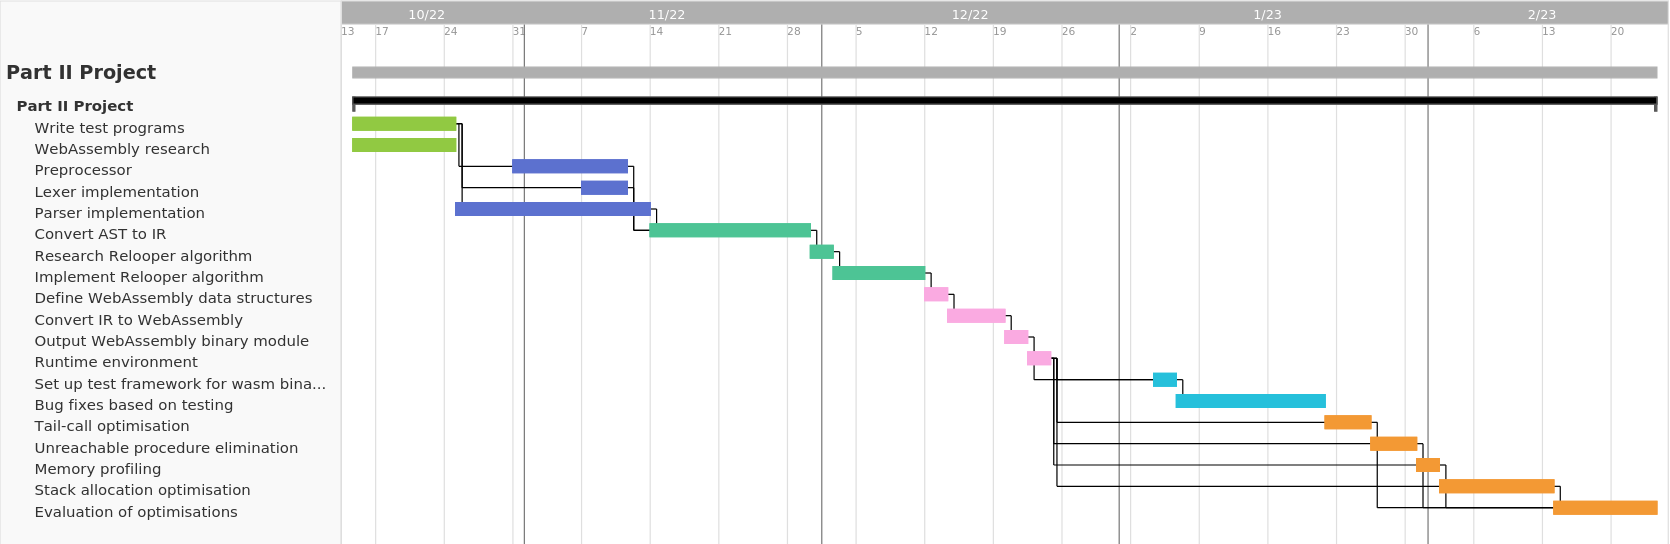
\includegraphics[width=0.95\textwidth]{20-gantt-chart/00-gantt-chart}
  \caption{Gantt chart showing dependencies between each task of the project. High-level sections are distinguished by colour: preparatory research, front end, middle end, back end, testing, and optimisations.}%
  \label{fig:gantt chart}
\end{figure}

I used Git as my version control system~\ccite{git}.
I regularly committed my code in small, revertible chunks, and pushed the repository to GitHub to maintain an up-to-date off-site backup~\ccite{github}.
\Ccref{fig:github contribution graph} shows a graph of my commits over time.
In the later stages of the project, I used pre-commit hooks to run automated tests on the project every time I committed, ensuring no inadvertent bugs were introduced.

\begin{figure}[t]
  \centering
  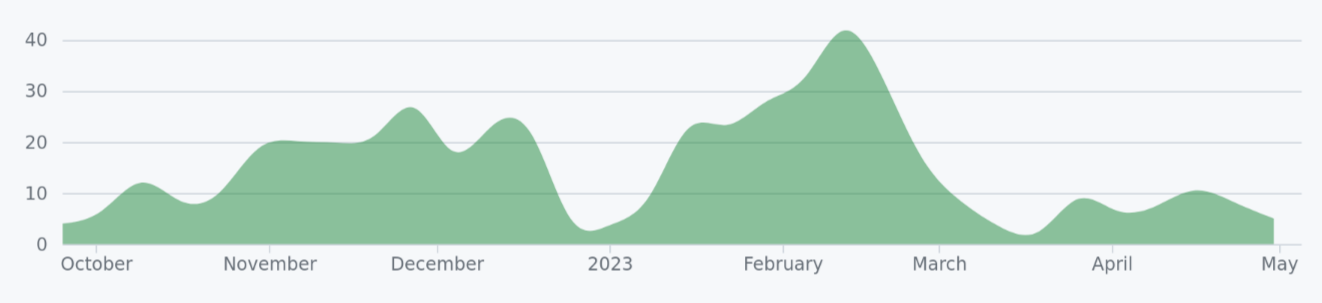
\includegraphics[width=0.8\textwidth]{12-github-commit-graph.png}
  \caption{My GitHub contribution graph, showing number of commits per week. Taken from my GitHub repository's ``Insights'' page.}%
  \label{fig:github contribution graph}
\end{figure}

Rather than use separate software for bug tracking, I decided to use tactile methods such as a physical notebook to record to-do lists and areas that needed work.
I was able to always have quick access to note down new bugs as well as staying on track with the current task.
I found this to be very helpful for staying focused and not getting distracted by other software.

\subsection{Testing}

% My testing strategy in the incremental model was to verify the correct functioning of each section, as much as possible, before moving onto the next section.
To facilitate testing, I wrote a suite of test programs designed to use different language constructs.
After completing each stage of the compiler pipeline, I carefully examined the output of compiling each test program, verifying its correctness.

Once the compiler could generate an \gls{ast}, I wrote a function to reconstruct the source code from the \gls{ast}.
I compared this output to the original source to confirm the program semantics were maintained.

When the entire pipeline was complete, I used GCC (the GNU Compiler Collection) as a reference compiler; I compiled my test programs with both my compiler and GCC, and verified that the resulting binaries produced the same output~\ccite{gcc}.

\section{Starting Point}

The \emph{Compiler Construction} course of the Tripos was the starting point for my knowledge of compilers.
The Part II \emph{Optimising Compilers} course was useful in extending my project with optimisations, though some of the optimisations I implemented went beyond the course.

I had familiarity with C from the \emph{Programming in C and C++} course, and from previous personal projects.
Additionally, I had experience writing JavaScript and Python from personal projects.
I gained all my knowledge of WebAssembly and Rust through independent research.


\section{Tools Used}

The main code for the compiler was written in Rust~\ccite{rust-lang}.
I wrote the runtime environment in JavaScript, using Node.js, which is necessary to interface with the Web\-Assembly binary~\ccite{javascript,nodejs}.
Additional development scripts, for automated testing and profiling, were written in Python, because of ease of use and my familiarity with libraries such as Matplotlib~\ccite{python,matplotlib}.

I used the LALRPOP parser generator library to generate parsing code from the abstract grammar of C~\ccite{lalrpop-docs}.
Other parser generator libraries are available for Rust: notably, \texttt{nom} and \texttt{pest}~\ccite{nom-parser,pest-parser}.
Originally \texttt{nom} was designed for parsing binary file formats, making it less suitable for parsing source code.
Another popular choice is \texttt{pest}, however it separates the formal grammar and \gls{ast} generation, making the code more complicated.
LALRPOP provides an intuitive and powerful approach, where each grammar rule contains both the grammar specification and code to generate the corresponding \gls{ast} node.

I used Git for version control with GitHub as an off-site backup, and the CLion IDE as my development environment using the Intellij Rust plugin~\ccite{git,github,clion,intellij-rust-plugin}.
Together they provide excellent support for Rust and C, including code analysis and debugging.


\section{Licensing}

LALRPOP is MIT licensed.
I have decided to also use the MIT license for my code.

\end{document}
